% ----------
% CONCLUSION
% ----------

% Defining TOC's sections before content
\section{Conclusion}

\begin{frame}
    \begin{center}
    \vspace{0.5cm}
    \boxed{
        Conclusion
    }
    \end{center}
\end{frame}

\begin{frame}
    \frametitle{Conclusion}
    \begin{itemize}
        \setlength\itemsep{1em}
        \item[$\diamond$] Description théorique relative aux méthodes de champ moyen pour le problème à N-corps
        \item[$\diamond$] Explication de la CDMFT, modification de la boucle d'auto-cohérence
        \item[$\diamond$] Vitesse, relations de symétrie entre les paramètres de bain
    \end{itemize}
    \vspace{0.5cm}
    \begin{colorblock}{Pistes}
        Études des symétries (théorie des groupes), minimisation des deux sous-bains en même temps.
    \end{colorblock}
\end{frame}

\begin{frame}
    \begin{center}
    \vspace{0.5cm}
    \boxed{
        Merci
    }
    \end{center}
\end{frame}

\begin{frame}
    \frametitle{Annexe - Fonction de distance $d$}
    La fonction de distance est donnée par
    \begin{align}
        d = \sum_{i\omega_n, \mu, \nu}W_n|(\vb{G}_c^{-1}(i\omega_n) - \vb{\Bar{G}}^{-1}(i\omega_n))_{\mu\nu}|^2,
        \label{eq: dist}
    \end{align}
    où $i\omega_n$ sont les fréquences de Matsubara et $W_n$ des poids arbitraires
    liés auxdites fréquences.
\end{frame}

\begin{frame}
    \frametitle{Annexe - Base mixte}
    La base mixte est une façon d'exprimer le problème,
    \begin{figure}
        \centering
        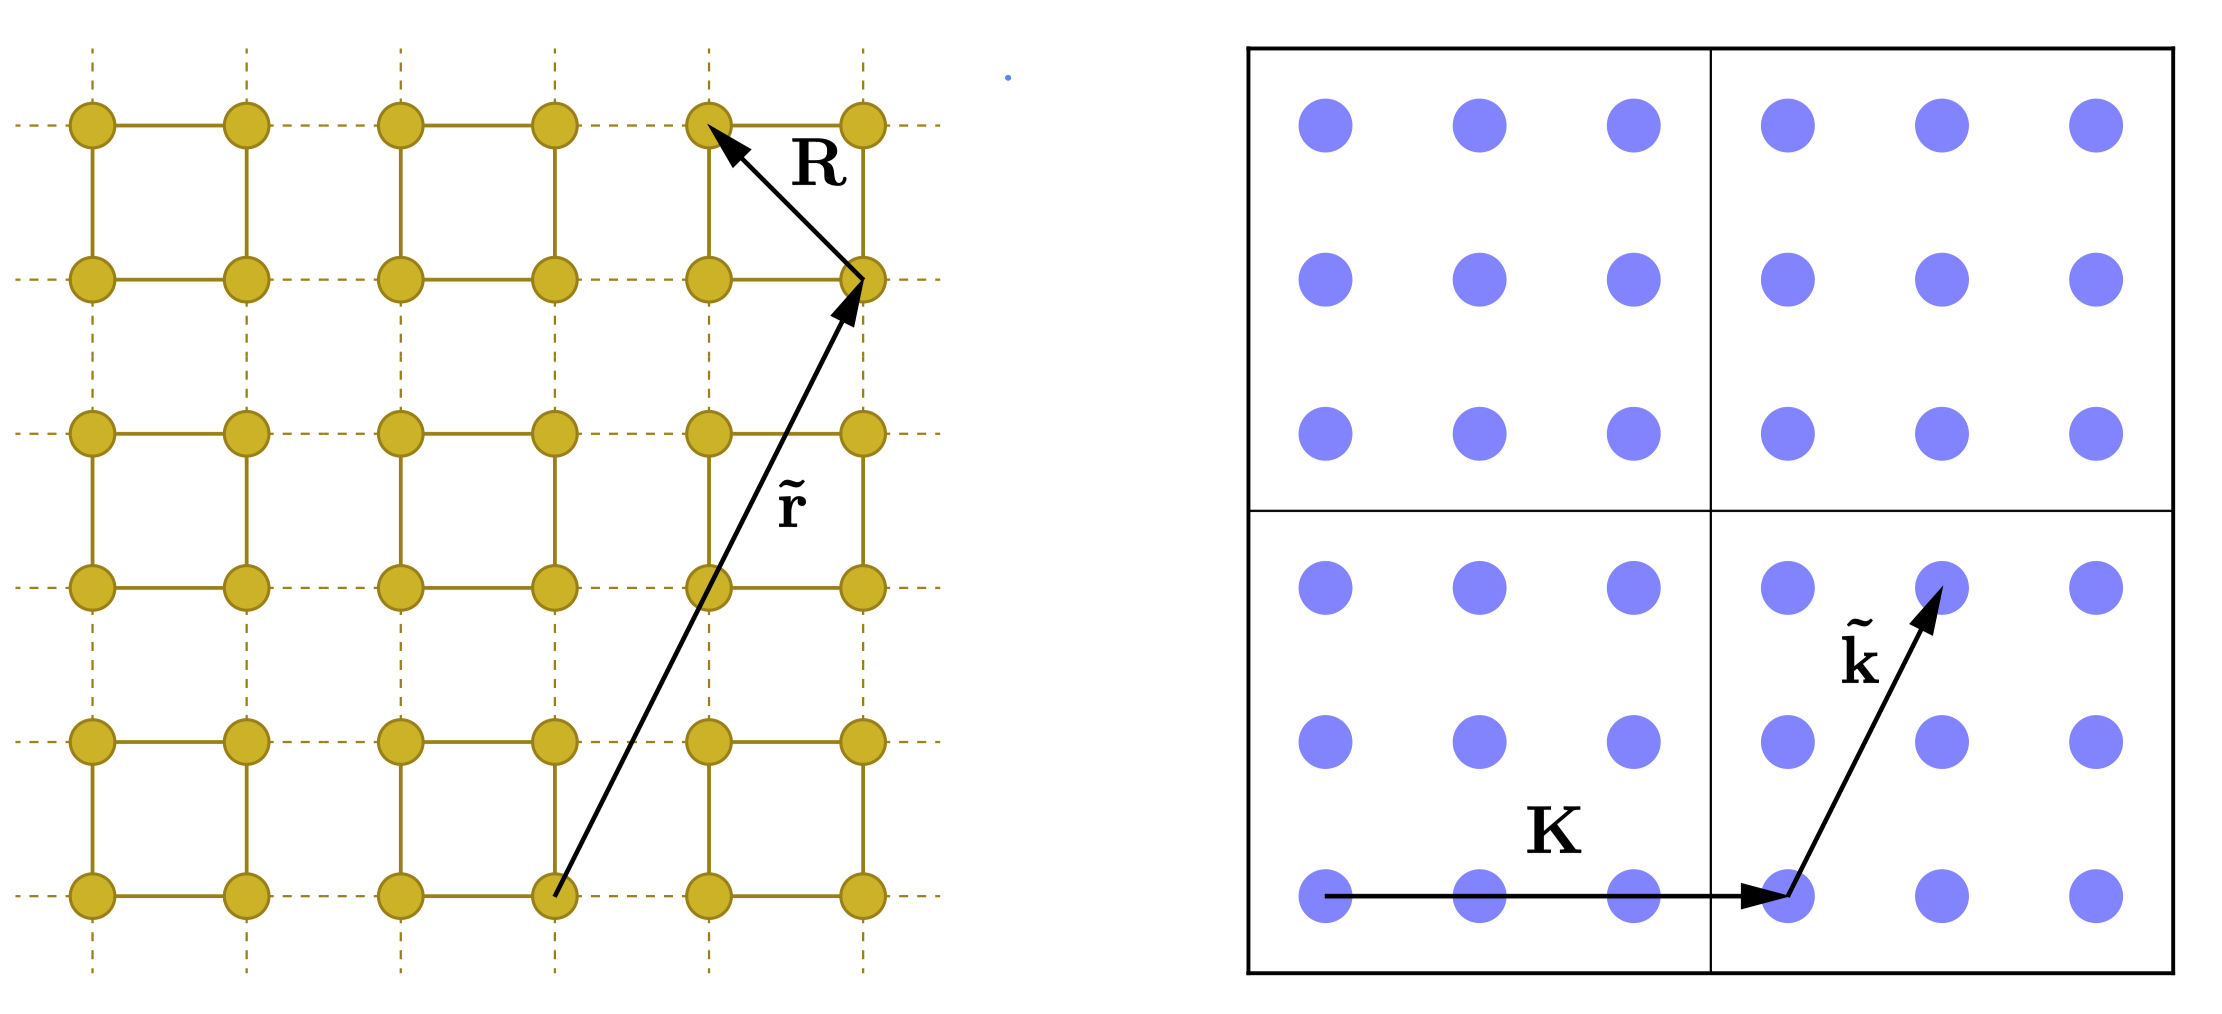
\includegraphics[scale=0.2]{./figures/theory/mixed_basis.png}
        \caption{(gauche) Réseau carré bidimensionnel découpé en amas dans la base des sites.
          (droite) Zone de Brillouin associée au réseau\footnotemark.}
        \label{fig: mixed_basis}
    \end{figure}
    \footnotetext{\textcolor{refs}{Maxime CHARLEBOIS.} “Théorie de champ moyen dynamique pour les systèmes
    inhomogènes”. \textcolor{sweet_refs}{Thèse de doct. Université Laval, 2015.}}
\end{frame}

\begin{frame}
    \frametitle{Annexe - Base mixte}
    Grâce aux transformée de Fourier partielles\footcite{MAIER}, on sépare
    les degrés de liberté inter-intra amas
    \begin{align}
      f(\vb{R}, \vb{\Tilde{r}}) &= \frac{N_c}{N}\sum_{\vb{\Tilde{k}}}e^{i\vb{\Tilde{k}}\cdot\vb{\Tilde{r}}}f(\vb{R}, \vb{\Tilde{k}})\\
      f(\vb{R}, \vb{\Tilde{k}}) &= \sum_{\vb{\Tilde{r}}}e^{-i\vb{\Tilde{k}}\cdot\vb{\Tilde{r}}}f(\vb{R}, \vb{\Tilde{r}}),
      \label{eq: partial_fourier}
    \end{align}
    \vfill
    \begin{noteblock}{Note}
      Le terme cinétique et la \textit{self-énergie} s'écrivent donc
      \begin{align*}
        \vb{\Sigma} = \vb{\Sigma}_c(\vb{R}, z) + \vb{\Sigma}(\vb{\tilde{k}}, z),
        &&\vb{t} = \vb{t}_c(\vb{R}) + \vb{t}(\vb{\tilde{k}})
      \end{align*}
    \end{noteblock}
\end{frame}
